\documentclass[tikz,border=3pt]{standalone}
\usepackage[utf8]{inputenc}
\usepackage[T1]{fontenc}
\usepackage{lmodern}
\renewcommand{\familydefault}{\sfdefault}
\usepackage{sansmath}\sansmath
\usepackage{chemfig}
\usepackage{pgfplots}\pgfplotsset{compat=1.18,/pgf/number format/use comma,/pgf/number format/1000 sep={.}}
\usetikzlibrary{arrows.meta,calc,positioning,decorations.pathmorphing,patterns}
% paleta del sitio
\definecolor{nar}{HTML}{E8680C}\definecolor{narc}{HTML}{FFB35C}\definecolor{hielo}{HTML}{FFF3E8}
\definecolor{tinta}{HTML}{1D1D1F}\definecolor{gris}{HTML}{6E6E73}\definecolor{lila}{HTML}{7C5CF0}
\definecolor{azul}{HTML}{2F6FD6}\definecolor{menta}{HTML}{17A673}\definecolor{coral}{HTML}{E8342A}
\begin{document}
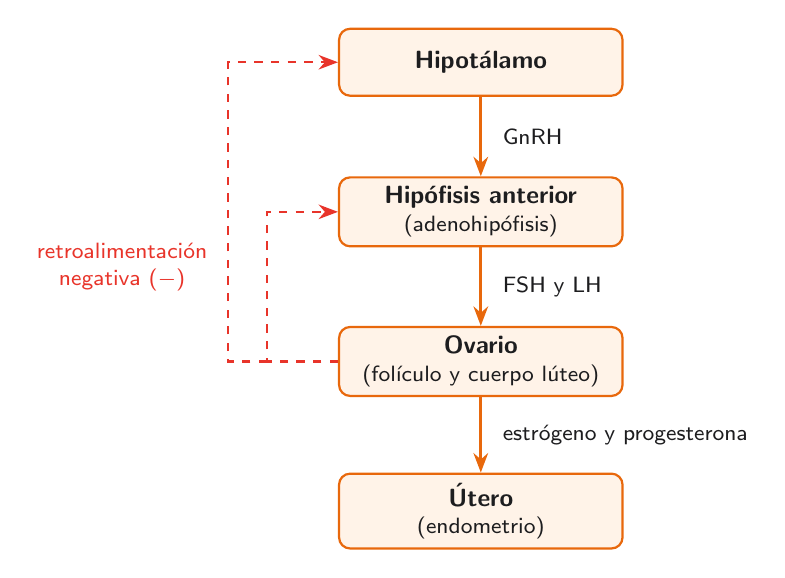
\begin{tikzpicture}[font=\small,
 caja/.style={draw=nar,thick,fill=hielo,rounded corners=4pt,minimum width=3.6cm,minimum height=0.85cm,align=center,text=tinta},
 fl/.style={-{Stealth[length=7pt]},very thick,nar},
 hor/.style={anchor=west,text=tinta,font=\footnotesize,align=left}]
\node[caja] (hip) at (0,0) {\textbf{Hipotálamo}};
\node[caja] (hipo) at (0,-1.9) {\textbf{Hipófisis anterior}\\[-1pt]\footnotesize(adenohipófisis)};
\node[caja] (ov) at (0,-3.8) {\textbf{Ovario}\\[-1pt]\footnotesize(folículo y cuerpo lúteo)};
\node[caja] (ut) at (0,-5.7) {\textbf{Útero}\\[-1pt]\footnotesize(endometrio)};
\draw[fl] (hip) -- (hipo) node[midway,hor,xshift=4pt] {GnRH};
\draw[fl] (hipo) -- (ov) node[midway,hor,xshift=4pt] {FSH y LH};
\draw[fl] (ov) -- (ut) node[midway,hor,xshift=4pt] {estrógeno y progesterona};
\draw[-{Stealth[length=7pt]},thick,coral,dashed] (ov.west) -- ++(-0.9,0) |- (hipo.west);
\draw[-{Stealth[length=7pt]},thick,coral,dashed] (ov.west) ++(-0.9,0) -- ++(-0.5,0) |- (hip.west);
\node[text=coral,font=\footnotesize,align=center,anchor=east] at (-3.35,-2.6) {retroalimentación\\negativa ($-$)};
\end{tikzpicture}
\end{document}
